\chapter{Trace analysis}

\section{Parsing}
Although the format presented in chapter \ref{v8-instrumentation} is really simple, parsing it can prove to be challenging.
The sole reason is the size of the files. It is really common for websites to produce files of size in the range of a few Gigabytes.
Some can even output as much as 48 GB in about 2 minutes!

The analyzing program was written in Haskell \cite{haskell:main-page}.
Haskell is a purely functional, lazy, statically typed language.
It has been chosen because it is relatively easy to write parsers in a language like this.
Further, static typing with pattern matching proves convenient when manipulating well-structured data like log entries.
Last but not least, automatically derived instances
\footnote{Without going into details, classes in Haskell are a bit like interfaces in 
object-oriented languages, e.g. class \emph{Ord} defines objects that can be compared}
help avoid writing tedious code and focus on implementing non-trivial parts.

All that being said, Haskell is a bit like C++ -- inexperienced user can easily make mistakes
that render the code slow and memory-greedy.

The logging format was described in section \ref{v8-bytecode-injection}.
Each entry consist of event type, and several locations. Each location comprises
function name, source file and position in the file.

At first, internal format for the event was exactly the same. One object consisted of
two strings and two numbers (it could be one number, but this way line and column info
logging can be turned on any time).

The first mistake, specific to Haskell, was to use \emph{String} type to represent function and file
names. The use of default \emph{String} to represent textual data makes the code inefficient 
because it is a linked lists of \emph{Char}s, i.e. to store one character 9 bytes of memory are used.
It is so wrong and inefficient to use this type that it is not worth trying to profile such implementation.

That error was fixed by changing the representation to \emph{ByteString} type from \emph{bytesting} 
package \cite{haskell:bytestring}. \emph{ByteString}s are represented internally as real byte arrays,
not linked lists. 
This change was accompanied by rewrite of the parsing code to \emph{attoparsec} \cite{haskell:attoparsec},
which can operate of \emph{ByteString}s as an input.

The code was now much less memory-consuming and faster, but it still seemed to consume too much memory.
Profiling proved that suspicions were warranted. The profiling diagram is shown on figure \ref{fig:bytestring-lazy}. 
All profiling diagrams in this section were collected by running the analyzing program on the same set of 6 input files.
First three occupy 48MB each, the last three 4MB each.
All files combined occupy around 150MB, while peak memory usage of the program is above 900MB.

\begin{figure}[hbt!]
 \centering
 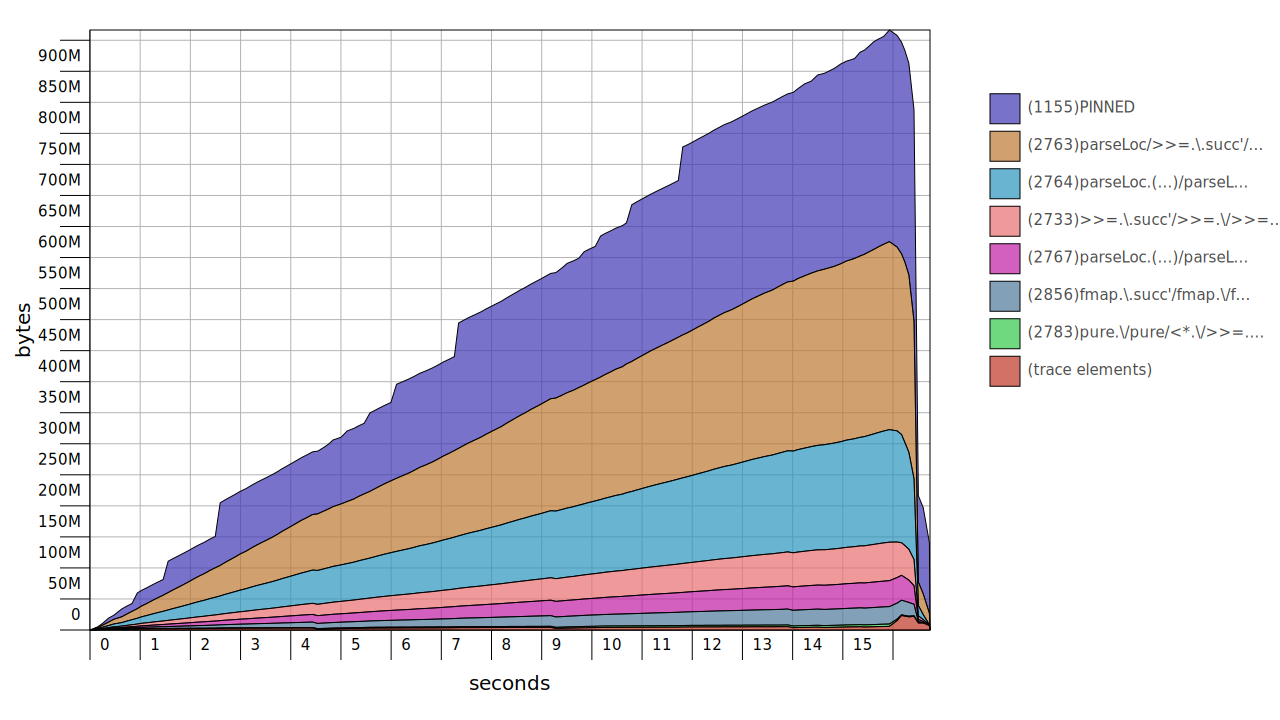
\includegraphics[width=\textwidth]{png/bytestring-lazy}
 \caption{Memory usage of the first implementation using ByteStrings as internal strings representation}
 \label{fig:bytestring-lazy}
\end{figure}

Looking at the diagram, pinned memory seemed to be never freed during the execution. 
Also, traces seemed to reside in memory for too long and occupy too much space. 

The first problem was a reflection of how Haskell keeps \emph{ByteString}s.
They are stored in pinned memory, which is kept on a heap but 
not managed by garbage collector \cite{haskell:shortbytestring-and-text} and cannot be moved around.
As a result, it leads to fragmentation of the heap and cannot be effectively managed.
The fix turned out to be simple. There is a more suitable storage format -- \emph{ShortByteString} 
(also part of the \emph{bytestring} package). It is managed
by GC and stored just like usual heap object, which can be moved around and easily garbage collected.
\footnote{So why even use \emph{ByteString}? Because it is stored in pinned memory, it can be passed to foreign functions.
Also, it is more efficient when the strings are really long and have long livespan}

The second problem was harder to track down. This time the cause was the laziness.
Laziness can improve the perfomance when some objects are never used and the language never needs to fully compute them. 
However, when we know that all objects will eventually be used, it is more efficient
to calculate them as soon as possible. The enforcement of eager evaluation seems to be an obscure
feature, but when we know what is going on, it is fine.
The improvement was visible (figure \ref{fig:shortbytestring-strict}) but it was not the end, 
as peak usage of almost 240MB is still greater than 150MB.

\begin{figure}[hbt!]
 \centering
 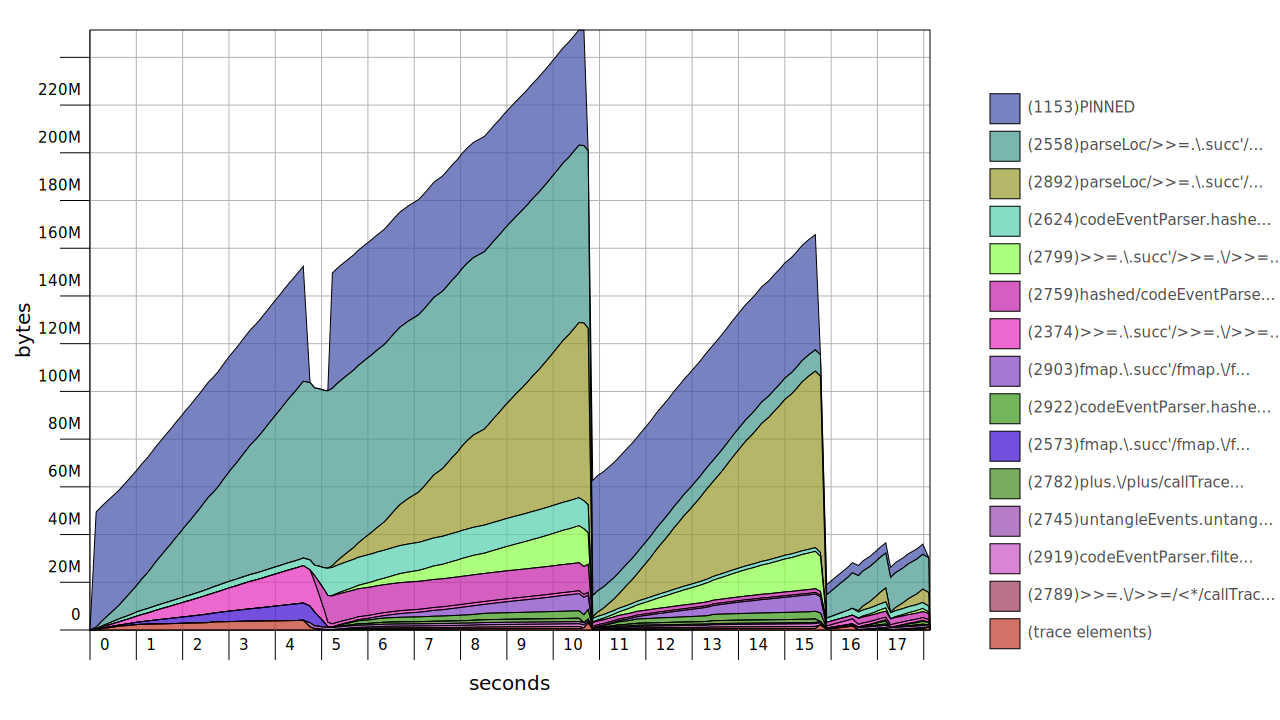
\includegraphics[width=\textwidth]{png/shortbytestring-strict}
 \caption{Memory usage after switching to ShortByteString and forcing eager evaluation}
 \label{fig:shortbytestring-strict}
\end{figure}

It seems suspicious that the entire file has to be kept in memory to be parsed 
(pinned memory on figure \ref{fig:shortbytestring-strict} represents input files read into memory). 
After all, if it was written in C++, probably one line at a time would be read and processed. 
So why this parser consumes so much memory?

This is what \emph{attoparsec} states about incremental input:

\begin{displayquote}
Note: incremental input does not imply that attoparsec will release portions of its internal state for 
garbage collection as it proceeds. Its internal representation is equivalent to a single ByteString: 
if you feed incremental input to a parser, it will require memory proportional to the amount of input you supply. 
(This is necessary to support arbitrary backtracking.)
\end{displayquote}

So, our parser keeps the whole file contents in memory to be able to backtrack. But it is not necessary with
such a simple format. Fortunately, it is possible to improve this behaviour.
Currently, the parser tries to parse the entire file into a list of events. To be sure that it can backtrack,
it keeps the whole input in memory. Instead, we can ask the parser to parse only one event. 
It will do it and return the part of the input that was not parsed yet. We can repeat that in a loop
and parser will never keep more memory that just a few kilobytes. 
Figure \ref{fig:single-event} shows the improvement.

\begin{figure}[hbt!]
 \centering
 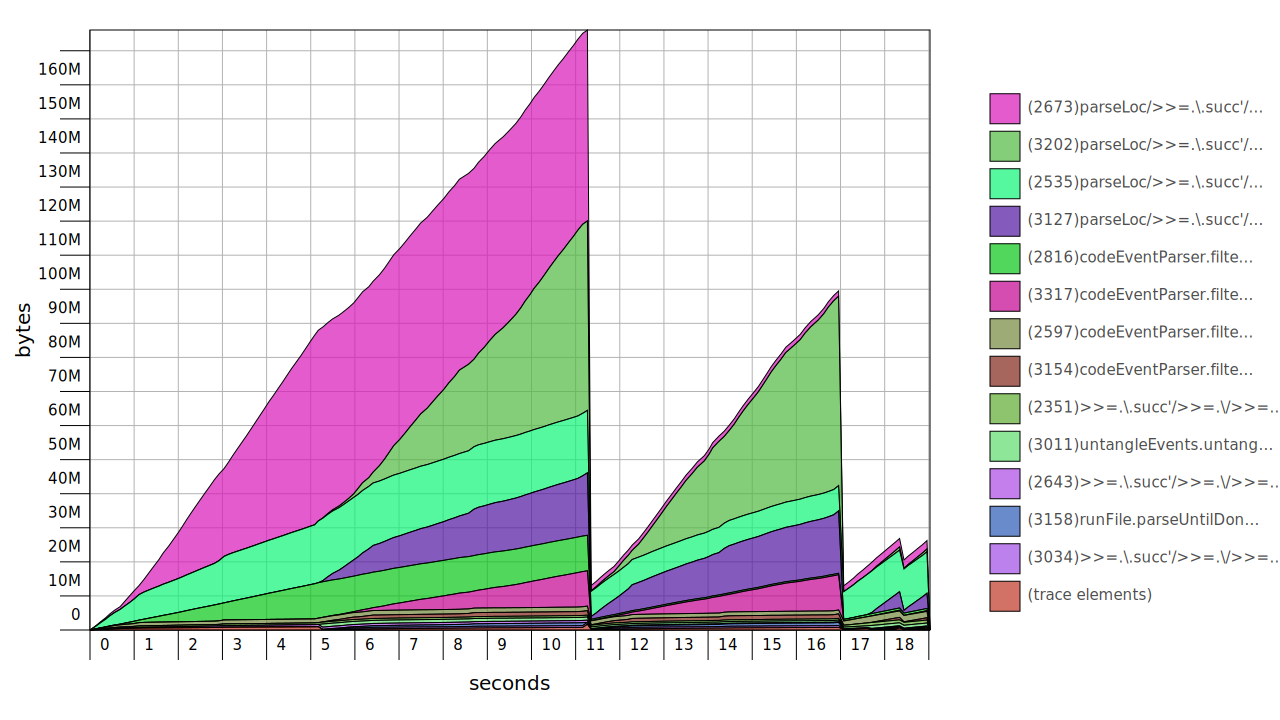
\includegraphics[width=\textwidth]{png/single-event}
 \caption{Memory usage after preventing parser from keeping the entire input file in the memory}
 \label{fig:single-event}
\end{figure}

Last, but not least, the internal representation of the event can be greatly improved.
Locations consist of file names and function names. But both sets are limited!
Usualy there are only a few sources containing just a few hundreds of unique functions. 
We can create a map of all source and function names and just keep appropriate ids in location objects.
Just 4 numbers instead of 2 strings and 2 numbers!

This representation also has another major benefit -- comparisons of such objects are much fasters.

The final memory consumption is presented in figure \ref{fig:strings-map}

\begin{figure}[hbt!]
 \centering
 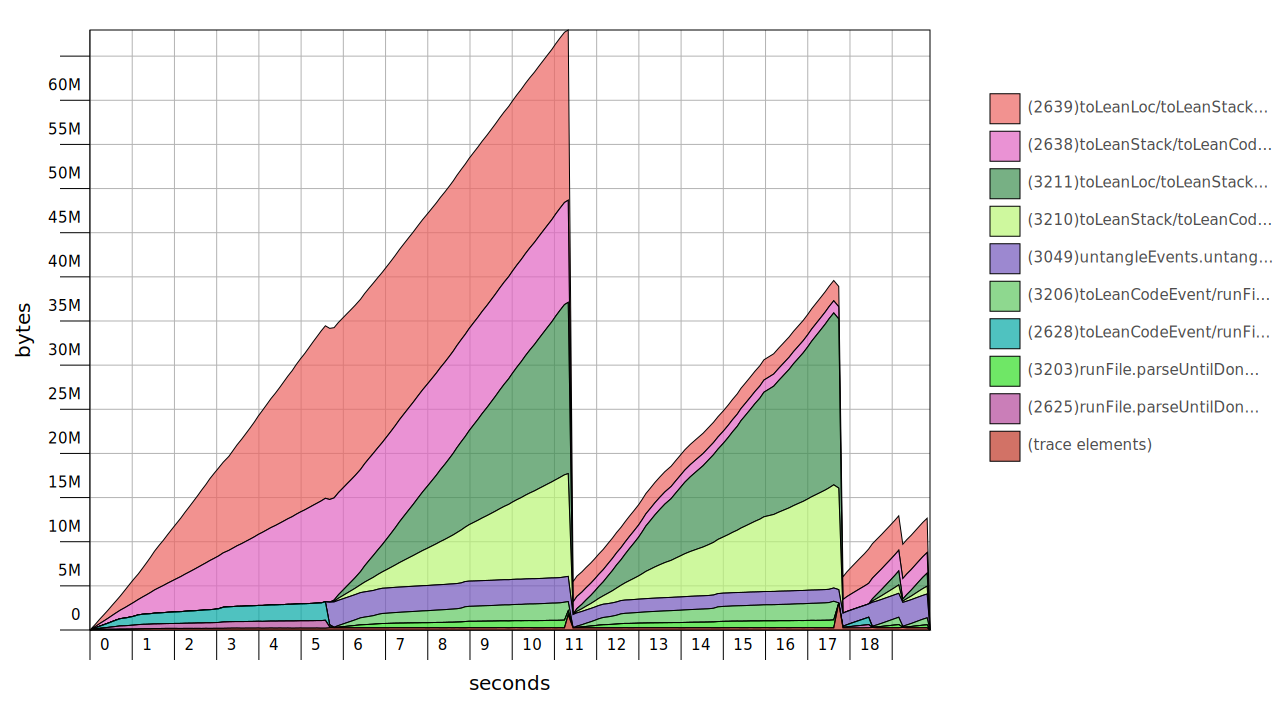
\includegraphics[width=\textwidth]{png/strings-map}
 \caption{Final memory usage}
 \label{fig:strings-map}
\end{figure}


\section{Trace untangling}
Due to the nature of JavaScript execution model (see section \ref{js-exec-model}), execution events
corresponding to different JavaScript events or functions can be intertwined.

For this reason, all events forming a trace have to be untangled into subtraces, each corresponding
to one script or callback. 

Let us recall that all events are logged by our instumented Chromium with their call stacks.
Now, we have three cases:
\begin{itemize}
  \item The event is a function enter with an empty call stack -- it starts a new subtrace
  \item The event is a function exit removing the last item from the stack -- it ends a subtrace
  \item Any other event -- it is a continuation of a subtrace, whose last event has the same call stack
\end{itemize}

Naturally, some care has to be taken to ensure that the right stack is compared. Some events change the
call stack, e.g. function enter and exit, some do not, e.g. "if statement -- then".
Here, the stack \emph{after} the event occured is saved and it is appopriately modified 
(one location can be added, removed or nothing is changed) when comparing
with past events stacks.

Listing \ref{alg-untangling} presents the pseudocode of the algorithm.

\lstinputlisting[language=Pseudocode, caption=Trace untangling, label=alg-untangling, mathescape=true]{algorithms/untangling.alg}

The above code is rather uncomplicated, but it is slow when implemented naively.
The most wasteful part is finding the trace with the right stack in \emph{findMatchingSubtrace}.
To make it faster, two things were done:
\begin{itemize}
  \item Location objects are just 4 numbers instead of 2 strings and 2 numbers. This makes stack comparisons
           one or two orders of magnitude faster
  \item Open traces are kept in a map indexed by stack of the last event. 
  			The lookup becomes logarithmic instead of linear. This optimization is especially important when there are lots
  			of intertwined subtraces. It also must be noted that this optimization alone would not help much if the comparisons 
  			between stacks were slow
\end{itemize} 

\section{Trace alignment}
\label{trace-alignment}

\cite{ieee:alignment-and-slicing}

\section{Trace matching using SMP}

\section{Noise filtering}


